\chapter{Specific Requirements}

\section{External Interface Requirements}

\subsection{User Interfaces}
\subsection{Hardware Interfaces}
\subsection{Software interfaces}
\subsection{Communications Interfaces}

\section{Functional Requirements}

\subsection{Requirements}

\subsection{Definition of Use Case Diagrams}

Bla bla bla...

\begin{figure}[H]
	\centering
	% \captionsetup{justification=centering,margin=1cm}

	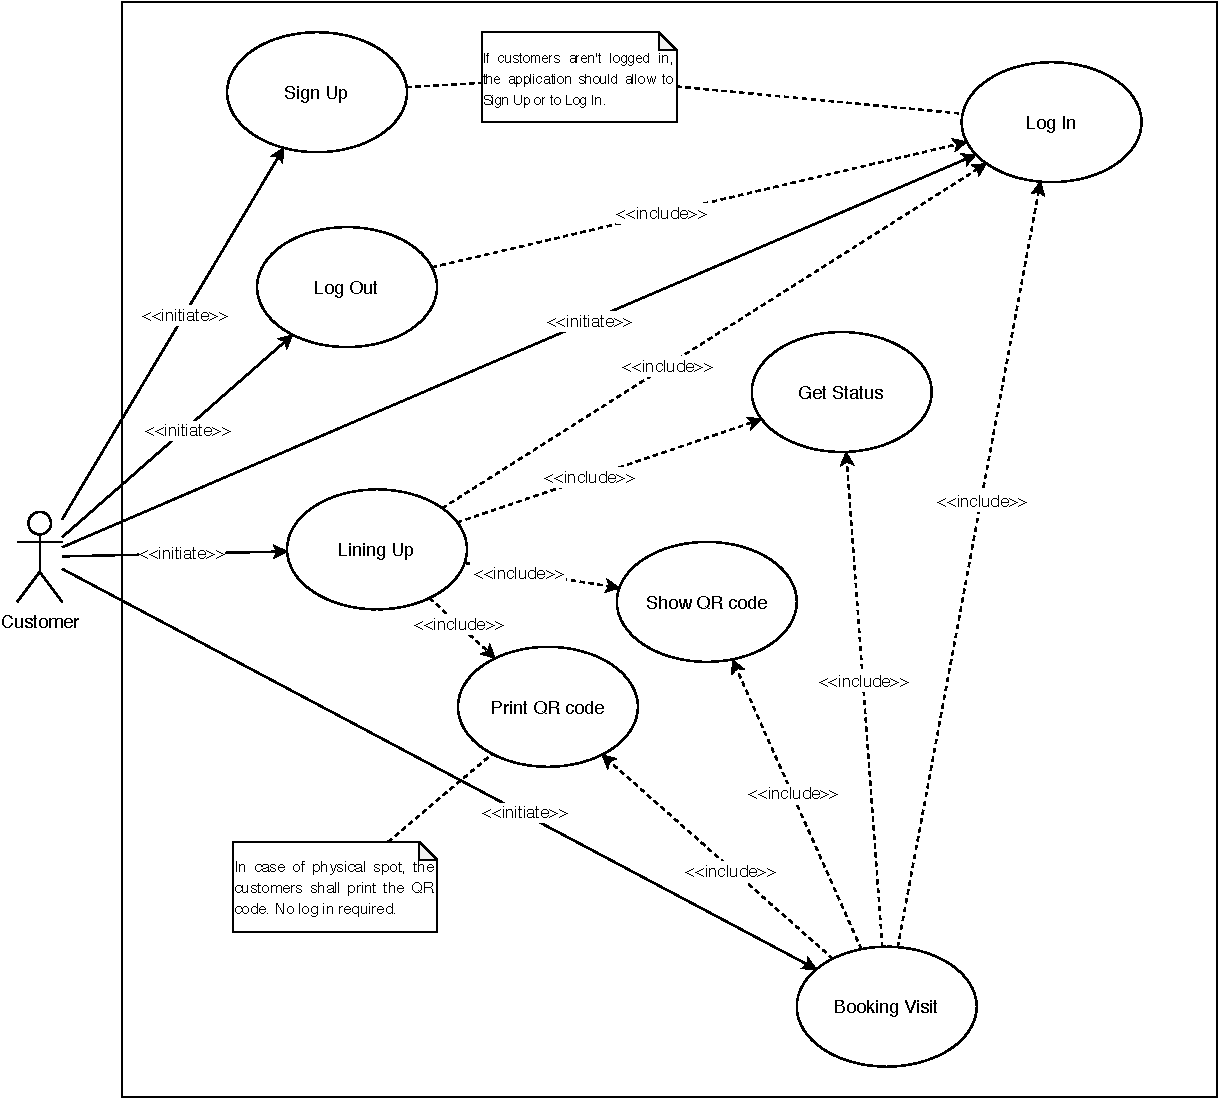
\includegraphics[width=1.0\textwidth]{images/customers_use_cases_diagram.pdf}
	\caption{Customers use cases diagram.}
	\label{customersUseCasesDiagram}
\end{figure}

\begin{table}[h!]
\centering
\begin{tabular}{| m{0.3\textwidth} | m{0.7\textwidth} |} 
	\hline
	\textbf{Name} & Sign Up \\ 
	\hline
	\textbf{Actor} & Customer \\ 
	\hline
	\textbf{Entry Conditions} & Customer is on the Sign Up page. \\ 
	\hline
	\textbf{Event Flows} &
	\begin{itemize}
		\item Customer inserts the requested information in the form.
		\item Customer clicks on the Sign Up button.
	\end{itemize} \\ 
	\hline
	\textbf{Exit Conditions} & Sign Up completed successfully and customer is logged in. \\ 
	\hline
	\textbf{Exceptions} &
	\begin{itemize}
		\item Customer's username already in use.
		\item Empty form field.
		\item Policy agreement rejected.
		\item Lost Internet connection.
	\end{itemize} \\ 
	\hline
\end{tabular}
\caption{Customer - use case: \textbf{Sign Up}.}
\label{tableSignUp}
\end{table}

\begin{table}[h!]
\centering
\begin{tabular}{| m{0.3\textwidth} | m{0.7\textwidth} |} 
	\hline
	\textbf{Name} & Log In \\ 
	\hline
	\textbf{Actor} & Customer \\ 
	\hline
	\textbf{Entry Conditions} & Customer is on the Log In page. \\ 
	\hline
	\textbf{Event Flows} &
	\begin{itemize}
	\item Customer inserts the requested information in the form.
	\item Customer clicks on the Log In button.
	\end{itemize} \\ 
	\hline
	\textbf{Exit Conditions} & Log In completed successfully. \\ 
	\hline
	\textbf{Exceptions} &
	\begin{itemize}
	\item Customer's username or password incorrect.
	\item Empty form filed.
	\item Lost Internet connection.
	\end{itemize} \\ 
	\hline
\end{tabular}
\caption{Customer - use case: \textbf{Log In}.}
\label{tableLogIn}
\end{table}

\begin{table}[h!]
\centering
\begin{tabular}{| m{0.3\textwidth} | m{0.7\textwidth} |} 
	\hline
	\textbf{Name} & Log Out \\ 
	\hline
	\textbf{Actor} & Customer \\ 
	\hline
	\textbf{Entry Conditions} & Customer is on the Log Out page. \\ 
	\hline
	\textbf{Event Flows} &
	\begin{itemize}
	\item Customer clicks on the Log Out button.
	\end{itemize} \\ 
	\hline
	\textbf{Exit Conditions} & Log Out completed successfully. \\ 
	\hline
	\textbf{Exceptions} &
	\begin{itemize}
	\item Customer already logged out.
	\item Lost Internet connection.
	\end{itemize} \\ 
	\hline
\end{tabular}
\caption{Customer - use case: \textbf{Log Out}.}
\label{tableLogIn}
\end{table}


\subsection{Use Cases and Sequence/Activity Diagrams}
\subsection{Mapping on Requirements}

\section{Performance Requirements}

\section{Design Constraints}

\subsection{Standard Compliance}
\subsection{Hardware limitations}
\subsection{Any Other Constraint}

\section{Software System Attributes}

\subsection{Reliability}
\subsection{Availability}
\subsection{Security}
\subsection{Maintainability}
\subsection{Portability}